% !TeX root = ../Thesis.tex
\documentclass[../Thesis.tex]{subfiles}
\graphicspath{{\subfix{../images/}}}

\begin{document}

\section{Deadlocks}

Deadlocks are a common problem that can occur in concurrent systems,
which are systems where multiple threads or processes are
running simultaneously and potentially sharing resources.
They have been studied at least since \cite{dijkstra1964},
who coined the term ``deadly embrace'' in Dutch, which did not catch on.

A deadlock occurs when two or more threads or processes
are blocked and unable to continue executing
because each is waiting for the other to release a resource that it needs.
This results in a situation where none of the threads or processes
can make progress and the system becomes effectively stuck.
An alternative equivalent definition of deadlocks
in terms of program states can be found in \cite{holt1972some}.

Deadlocks can be a serious problem in concurrent systems,
as they can cause the system to become unresponsive or even crash.
Therefore, it is important to be able to detect and prevent deadlocks.
They can occur in any concurrent system where multiple threads or processes
are competing for shared resources.
Examples of shared resources that can lead to deadlocks include system memory,
input/output devices, locks, and other types of synchronization primitives.

Deadlocks can be difficult to detect and prevent
because they depend on the precise timing of events in the system.
Even in cases where deadlocks can be detected, resolving them can be difficult,
as it may require releasing resources that have already been acquired or
rolling back completed transactions.
To avoid deadlocks, it is important to carefully
manage shared resources in a concurrent system.
This can involve using techniques such as resource allocation algorithms,
deadlock detection algorithms, and other types of synchronization primitives.
By carefully managing shared resources,
it is possible to prevent deadlocks from occurring and
ensure the smooth operation of concurrent systems.

To understand the concept in more detail,
consider a simple example where two processes, A and B,
are competing for two resources, X and Y.
Initially, process A has acquired resource X and is waiting to acquire resource Y,
while process B has acquired resource Y and is waiting to acquire resource X.
In this situation, neither process can continue executing
because it is waiting for the other process to release a resource that it needs.
This results in a deadlock, as neither process can make progress.
Fig. \ref{fig:state-graph-example} illustrates this situation.
The cycle therein indicates a deadlock, as will be explained in the next section.



\begin{figure}[!htb]
      \centering
      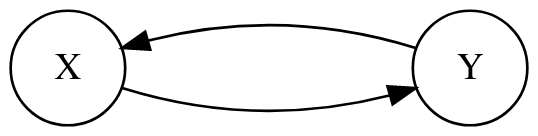
\includegraphics[scale=0.25]{state-graph-example.png}
      \caption{Example of a state graph with a cycle indicating a deadlock.}
      \label{fig:state-graph-example}
\end{figure}
\subsection{Necessary conditions}
\label{sec:coffman-conditions}

According to the classic paper on the topic \cite{coffman1971deadlocks},
the following conditions need to hold for a deadlock to arise.
They are sometimes called ``Coffman conditions''.

\begin{enumerate}
      \item \textbf{Mutual Exclusion}: At least one resource in the system must
            be held in a non-sharable mode, meaning that only one thread or process can use it at a time
            (e.g. a variable behind a mutex).
      \item \textbf{Hold and Wait}: At least one thread or process in the system must
            be holding a resource and waiting to acquire additional resources
            that are currently being held by other threads or processes.
      \item \textbf{No Preemption}: Resources cannot be preempted, which means that a thread or process
            holding a resource cannot be forced to release it until it has completed its task.
      \item \textbf{Circular Wait}: There must be a circular chain of two or more threads or processes,
            where each thread or process is waiting for a resource held by the next one in the chain.
            This is usually visualized in a graph representing the order in which the resources are acquired.
\end{enumerate}

Usually, the first three conditions are characteristics of the system under study, i.e.
the protocols used for acquiring and releasing resources,
while the fourth may or may not occur depending
on the interleaving of instructions during the execution.

It is worth noting that the Coffman conditions are in general necessary
but not sufficient for a deadlock to occur.
The conditions are indeed sufficient in the case of single-instance resource systems.
But they only indicate the possibility of deadlock in systems
where there are multiple indistinguishable instances of the same resource.

In the general case, if any one of the conditions is not met, a deadlock cannot occur,
but the presence of all four conditions does not necessarily guarantee a deadlock.
Nonetheless, the Coffman conditions are an important tool for understanding and
analyzing the causes of deadlocks in concurrent systems
and they can help guide the development of strategies for preventing and resolving deadlocks.

\subsection{Strategies}

Several strategies for handling deadlocks exist,
each of which has its strengths and weaknesses.
In practice, the most effective strategy will depend on the specific requirements
and constraints of the system being developed.
Designers and developers must carefully consider the trade-offs between different strategies
and choose the approach that is best suited to their needs.
Interested readers are referred to \cite{coffman1971deadlocks,singhal1989deadlock}.

\subsubsection{Prevention}

One way to deal with deadlocks is to prevent them from occurring in the first place.
The idea is for deadlocks to be excluded a priori.
With this objective in mind, we must ensure that at every point in time
at least one of the necessary conditions developed in Sec. \ref{sec:coffman-conditions}
is not satisfied.
This restricts the possible protocols in which requests for resources may be made.
We will now look at each condition in isolation
and elaborate on the most common approaches.

If the first condition must be false,
then the program should allow shared access to all resources.
Lock-free synchronization algorithms may be used for this purpose
since they do not implement mutual exclusion.
This is difficult to achieve in practice for all resource types,
since for example a file may not be shared by more than one thread or process
during an update of the file contents.

Looking at the second condition, a feasible approach would be to impose that
each thread or process acquires all the required resources at once and that
the thread or process can not proceed until access to all of them has been granted.
This all-or-nothing policy causes a significant performance penalty,
given that resources may be allocated to a specific thread or process
but may remain unused for long periods.
In simpler terms, it decreases concurrency.

If the no preemption condition is denied, then resources may be recovered
in certain circumstances, e.g. using resource allocation algorithms that
ensure that resources are never held indefinitely.
After a timeout or when a condition is satisfied,
the thread or process releases the resource
or a supervisor process recovers the resource forcibly.
Usually, this works well when the state of the resource can be easily saved
and restored later.
One example of this is the allocation of CPU cores in a modern operating system.
The scheduler allocates one processor core to one task and
may switch to a different task or
move the task to a new processor core at any moment just
by saving the contents of the registers \cite[Chapter 6]{ArpaciDusseau2018}.
However, if preserving the resource state is not possible,
preemption may entail a loss of the progress done so far,
which is not acceptable in many scenarios.

Lastly, if the state graph of the resources never forms a cycle,
then the fourth necessary condition is false and deadlocks are prevented.
To achieve this one could introduce a linear ordering of resource types.
In other words, if a process or thread has been allocated resources of type $r_i$,
it may subsequently require only those resources
of types that follow $r_i$ in the ordering.
This involves using special synchronization primitives
that allow resources to be shared in a controlled manner and
enforcing strict rules for resource acquisition and release.
Under these conditions, the state graph will be strictly speaking
a forest (an acyclical graph) and no deadlocks are possible.

In practical applications, a combination of the previous strategies may prove useful
when none of them is entirely applicable.
\subsubsection{Avoidance}

Avoidance is another strategy for dealing with deadlocks,
which involves dynamically detecting and
avoiding potential deadlocks \emph{before} they occur.
For this, the system requires global knowledge in advance regarding
which resources a thread or process will request during its lifetime.
Note that, in linguistic terms,
``deadlock avoidance'' and ``deadlock prevention'' may seem similar,
but in the context of deadlock handling, they are distinct concepts.

One of the classic deadlock avoidance algorithms
is the Banker's algorithm \cite{dijkstra1964}.
Another relevant algorithm is proposed by \cite{habermann1969prevention}.

Regrettably, these techniques are only effective in highly specific scenarios,
such as in an embedded system where the complete set of tasks to be executed
and their required locks are known a priori.
Consequently, deadlock avoidance is not a commonly used solution
applicable to a broad range of situations.

\subsubsection{Detection and Recovery}

Another strategy to handle deadlocks is to detect them
\emph{after} they occur and recover from them.
For a survey of algorithms for deadlock detection
in distributed systems, see \cite{singhal1989deadlock}.
We will briefly present the general idea behind one of them for illustration purposes.

The Resource Allocation Graph (RAG) is a commonly used method
for detecting deadlocks in concurrent systems.
It represents the relationship between threads/processes
and resources in the system as a directed graph.
Each process and resource is represented by a node in the graph
and a directed edge is drawn from a process to a resource
if the process is currently holding that resource.
This is analogous to the state graph shown in Fig. \ref{fig:state-graph-example}
but with the threads/processes represented in the diagram.
The state graph may also be applied to deadlock detection \cite{coffman1971deadlocks}.

To detect deadlocks using the RAG, we need to look for cycles in the graph.
If there is a cycle in the graph, it indicates that
a set of processes is waiting for resources
that are currently being held by other processes in the cycle.
Therefore no process in the cycle can make progress.

The recovery part of the process involves
terminating one of the threads or processes in the cycle.
This causes the resources to be released and
the other threads or processes are allowed to continue.

Numerous database management systems (DBMS)
incorporate subsystems for detecting and resolving deadlocks.
A deadlock detector is executed at intervals,
generating a regular allocation graph,
otherwise called the transaction-wait-for (TWF) graph,
and examining it for any cycles.
If a cycle (deadlock) is identified, the system must be restarted.
An excellent overview of deadlock detection
in distributed database systems is \cite{knapp1987deadlock}.
The subject of concurrency control and recovery from deadlocks in DBMSs is
extensively discussed in \cite{bernstein1987concurrency}.

\subsubsection{Acceptance or ignoring deadlocks altogether}

In some cases, it may be admissible
to simply accept the risk of deadlocks and manage them as they occur.
This approach may be appropriate in systems where the cost of preventing
or detecting deadlocks is too high, or where the frequency of deadlocks is low enough
that the impact on system performance is minimal,
or where the data loss incurred each time is tolerable.

UNIX is an example of an OS following this principle \cite[p. 477]{shibu2016}.
Other major operating systems also exhibit this behavior.
On the other hand, a life-critical system cannot afford
to pretend its operation will be deadlock-free for any reason.

\end{document}